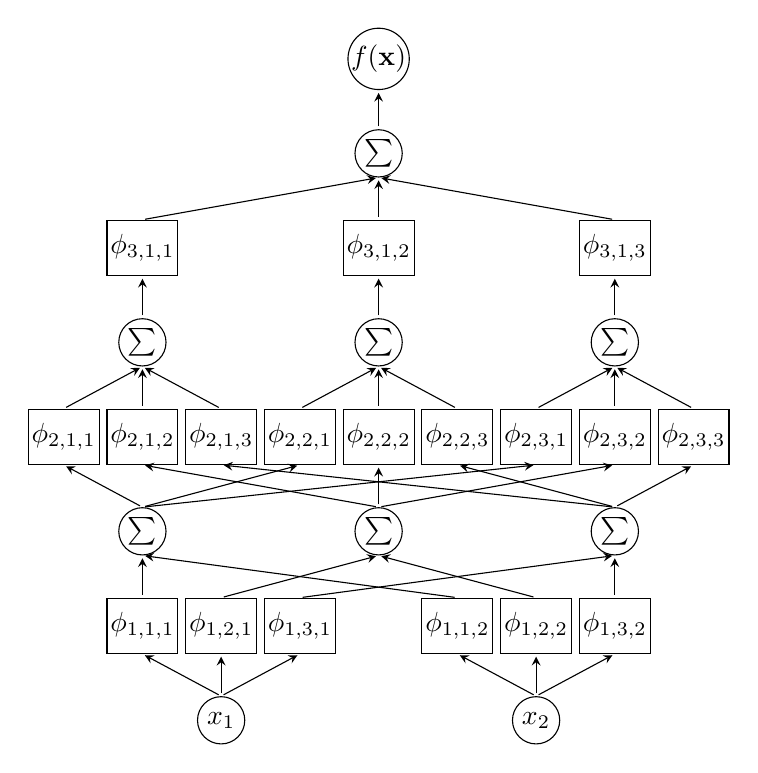
\begin{tikzpicture}[
	neuron/.style={circle, draw, minimum size=6mm, inner sep=0pt},
	box/.style={draw, rectangle, minimum width=9mm, minimum height=7mm, inner sep=1pt, fill=white},
	>=stealth
	]
	
	%-----------------------
	% Customizable heights (compact stack)
	%-----------------------
	\def\hin{0.0}        % inputs
	\def\hphiI{1.2}      % layer-1 phi_{1,p,q}
	\def\hsumI{2.4}      % first hidden sums (S1..S3)
	\def\hphiII{3.6}     % layer-2 phi_{2,r,q} (9 boxes)
	\def\hsumII{4.8}     % second hidden sums (T1..T3)
	\def\hphiIII{6.0}    % layer-3 phi_{3,1,r}
	\def\hsumall{7.2}    % global sum
	\def\hout{8.4}       % output
	
	%-----------------------
	% Row 1: inputs
	%-----------------------
	\node[neuron] (X1) at (-2,\hin) {$x_1$};
	\node[neuron] (X2) at ( 2,\hin) {$x_2$};
	
	%-----------------------
	% Row 2: layer-1 univariate functions phi_{1,p,q}
	% columns p=1..3 placed at xA,xB,xC; q=1 from x1 (left), q=2 from x2 (right)
	\node[box] (phi111) at (-3,\hphiI) {$\phi_{1,1,1}$};
	\node[box] (phi121) at (-2,\hphiI) {$\phi_{1,2,1}$};
	\node[box] (phi131) at (-1,\hphiI) {$\phi_{1,3,1}$};
	
	\node[box] (phi112) at (1,\hphiI) {$\phi_{1,1,2}$};
	\node[box] (phi122) at (2,\hphiI) {$\phi_{1,2,2}$};
	\node[box] (phi132) at (3,\hphiI) {$\phi_{1,3,2}$};
	
	%-----------------------
	% Row 3: first hidden sums S1..S3 (p = 1..3)
	%-----------------------
	\node[neuron] (S1) at (-3,\hsumI) {$\textstyle\sum$};
	\node[neuron] (S2) at (0,\hsumI) {$\textstyle\sum$};
	\node[neuron] (S3) at (3,\hsumI) {$\textstyle\sum$};
	
	%-----------------------
	% Row 4: layer-2 univariate functions phi_{2,r,q}
	% For each target r∈{1,2,3} (columns xA,xB,xC), we place three boxes fed by S1,S2,S3.
	% left/mid/right offsets correspond to q=1 from S1, q=2 from S2, q=3 from S3.
	\node[box] (phi211) at (-4,\hphiII) {$\phi_{2,1,1}$};
	\node[box] (phi221) at (-3,     \hphiII) {$\phi_{2,1,2}$};
	\node[box] (phi231) at (-2,\hphiII) {$\phi_{2,1,3}$};
	
	\node[box] (phi212) at (-1,\hphiII) {$\phi_{2,2,1}$};
	\node[box] (phi222) at (0,     \hphiII) {$\phi_{2,2,2}$};
	\node[box] (phi232) at (1,\hphiII) {$\phi_{2,2,3}$};
	
	\node[box] (phi213) at (2,\hphiII) {$\phi_{2,3,1}$};
	\node[box] (phi223) at (3,     \hphiII) {$\phi_{2,3,2}$};
	\node[box] (phi233) at (4,\hphiII) {$\phi_{2,3,3}$};
	
	%-----------------------
	% Row 5: second hidden sums T1..T3 (r = 1..3)
	%-----------------------
	\node[neuron] (T1) at (-3,\hsumII) {$\textstyle\sum$};
	\node[neuron] (T2) at (0,\hsumII) {$\textstyle\sum$};
	\node[neuron] (T3) at (3,\hsumII) {$\textstyle\sum$};
	
	%-----------------------
	% Row 6: layer-3 univariate functions phi_{3,1,r} (r feeds the single top unit)
	%-----------------------
	\node[box] (phi311) at (-3,\hphiIII) {$\phi_{3,1,1}$};
	\node[box] (phi312) at (0,\hphiIII) {$\phi_{3,1,2}$};
	\node[box] (phi313) at (3,\hphiIII) {$\phi_{3,1,3}$};
	
	%-----------------------
	% Row 7: global sum and Row 8: output
	%-----------------------
	\node[neuron] (Sall) at (0,\hsumall) {$\textstyle\sum$};
	\node[neuron] (F)    at (0,\hout)    {$f(\mathbf{x})$};
	
	%-----------------------
	% Connections (top/bottom anchors)
	%-----------------------
	\tikzset{connect/.style={->,shorten >=1pt,shorten <=1pt}}
	
	% Inputs -> layer-1 phi
	\draw[connect] (X1.north) -- (phi111.south);
	\draw[connect] (X1.north) -- (phi121.south);
	\draw[connect] (X1.north) -- (phi131.south);
	
	\draw[connect] (X2.north) -- (phi112.south);
	\draw[connect] (X2.north) -- (phi122.south);
	\draw[connect] (X2.north) -- (phi132.south);
	
	% layer-1 phi -> first hidden sums
	\draw[connect] (phi111.north) -- (S1.south);
	\draw[connect] (phi112.north) -- (S1.south);
	
	\draw[connect] (phi121.north) -- (S2.south);
	\draw[connect] (phi122.north) -- (S2.south);
	
	\draw[connect] (phi131.north) -- (S3.south);
	\draw[connect] (phi132.north) -- (S3.south);
	
	% first hidden sums S{1,2,3} -> layer-2 phi boxes for each target T{1,2,3}
	% Column r=1 (xA)
	\draw[connect] (S1.north) -- (phi211.south);
	\draw[connect] (S2.north) -- (phi221.south);
	\draw[connect] (S3.north) -- (phi231.south);
	% Column r=2 (xB)
	\draw[connect] (S1.north) -- (phi212.south);
	\draw[connect] (S2.north) -- (phi222.south);
	\draw[connect] (S3.north) -- (phi232.south);
	% Column r=3 (xC)
	\draw[connect] (S1.north) -- (phi213.south);
	\draw[connect] (S2.north) -- (phi223.south);
	\draw[connect] (S3.north) -- (phi233.south);
	
	% layer-2 phi -> second hidden sums T{1,2,3}
	\draw[connect] (phi211.north) -- (T1.south);
	\draw[connect] (phi221.north) -- (T1.south);
	\draw[connect] (phi231.north) -- (T1.south);
	
	\draw[connect] (phi212.north) -- (T2.south);
	\draw[connect] (phi222.north) -- (T2.south);
	\draw[connect] (phi232.north) -- (T2.south);
	
	\draw[connect] (phi213.north) -- (T3.south);
	\draw[connect] (phi223.north) -- (T3.south);
	\draw[connect] (phi233.north) -- (T3.south);
	
	% layer-3 phi -> global sum
	\draw[connect] (T1.north) -- (phi311.south);
	\draw[connect] (T2.north) -- (phi312.south);
	\draw[connect] (T3.north) -- (phi313.south);
	
	\draw[connect] (phi311.north) -- (Sall.south);
	\draw[connect] (phi312.north) -- (Sall.south);
	\draw[connect] (phi313.north) -- (Sall.south);
	
	% Global sum -> output
	\draw[connect] (Sall.north) -- (F.south);
	
\end{tikzpicture}
